\documentclass[a4paper, 11pt]{article}
    \usepackage[fontset = windowsnew]{ctex}
    \usepackage{geometry}
        \geometry{left=2.54cm,right=2.54cm,top=3.18cm,bottom=3.18cm}
    \usepackage{amsmath}
    \usepackage{amsfonts}
    \usepackage{amssymb}
    \usepackage{siunitx}
    \usepackage{booktabs}
    \usepackage{longtable}
    \usepackage{graphicx}
    \usepackage{subfig}
    \usepackage{float}
    \usepackage{fancyvrb}
    \usepackage[unicode]{hyperref}
    \usepackage{xcolor}
    \usepackage{cite}

    \usepackage{listings}
    \lstset{
        %行号
        numbers=left,
        %背景框
        framexleftmargin=10mm,
        frame=none,
        %背景色
        %backgroundcolor=\color[rgb]{1,1,0.76},
        backgroundcolor=\color[RGB]{245,245,244},
        %样式
        basicstyle=\ttfamily,
        keywordstyle=\bf\color{blue},
        numberstyle=\color[RGB]{0,192,192},
        commentstyle=\it\color[RGB]{0,96,96},
        stringstyle=\rmfamily\slshape\color[RGB]{128,0,0},
        %显示空格
        showstringspaces=false
    }

    %%%%%% 设置字号 %%%%%%
    \newcommand{\chuhao}{\fontsize{42pt}{\baselineskip}\selectfont}
    \newcommand{\xiaochuhao}{\fontsize{36pt}{\baselineskip}\selectfont}
    \newcommand{\yihao}{\fontsize{28pt}{\baselineskip}\selectfont}
    \newcommand{\erhao}{\fontsize{21pt}{\baselineskip}\selectfont}
    \newcommand{\xiaoerhao}{\fontsize{18pt}{\baselineskip}\selectfont}
    \newcommand{\sanhao}{\fontsize{15.75pt}{\baselineskip}\selectfont}
    \newcommand{\sihao}{\fontsize{14pt}{\baselineskip}\selectfont}
    \newcommand{\xiaosihao}{\fontsize{12pt}{\baselineskip}\selectfont}
    \newcommand{\wuhao}{\fontsize{10.5pt}{\baselineskip}\selectfont}
    \newcommand{\xiaowuhao}{\fontsize{9pt}{\baselineskip}\selectfont}
    \newcommand{\liuhao}{\fontsize{7.875pt}{\baselineskip}\selectfont}
    \newcommand{\qihao}{\fontsize{5.25pt}{\baselineskip}\selectfont}

\begin{document}
%%%% 定理类环境的定义 %%%%
\newtheorem{example}{例}             % 整体编号
\newtheorem{algorithm}{算法}
\newtheorem{theorem}{定理}[section]  % 按 section 编号
\newtheorem{definition}{定义}
\newtheorem{axiom}{公理}
\newtheorem{property}{性质}
\newtheorem{proposition}{命题}
\newtheorem{lemma}{引理}
\newtheorem{corollary}{推论}
\newtheorem{remark}{注解}
\newtheorem{condition}{条件}
\newtheorem{conclusion}{结论}
\newtheorem{assumption}{假设}
\newtheorem{problem}{问题}
%%%% 重定义 %%%%
\renewcommand{\contentsname}{目录}  % 将Contents改为目录
\renewcommand{\abstractname}{摘要}  % 将Abstract改为摘要
\renewcommand{\refname}{参考文献}   % 将References改为参考文献
\renewcommand{\indexname}{索引}
\renewcommand{\figurename}{图}
\renewcommand{\tablename}{表}
\renewcommand{\appendixname}{附录}

    \title{\textbf{AVL树$\rightarrow$红黑树问题}\\\xiaosihao \emph{《现代操作系统》实验报告}}
    \author{王晗\\(2013011076)}
    \date{\today}
    \maketitle
    %\tableofcontents
    %\newpage

    \section{实验内容}
        在Windows的虚拟内存管理中,将VAD组织成AVL树。VAD树是一种平衡二叉树。红黑树也是一种自平衡二叉查找树,在Linux 2.6及其以后版本的内核中,采用红黑树来维护内存块。

        请尝试参考Linux源代码将WRK源代码中的VAD树由AVL树替换成红黑树。

    \section{实验环境搭建}
        实验使用\texttt{VirtualBox 5.0.8}作为虚拟机控制台,安装\texttt{Windows Server 2003 SP1}用于内核的调试。配置虚拟机串口,连接到命名管道:$\mathtt{\backslash\backslash.pipe\backslash debugger}$。将编译后的内核程序\texttt{wrkx86.exe}和硬件抽象层动态链接库\texttt{halacpim.dll}放置在$\mathtt{C:\backslash Windows\backslash system32}$ 下,并向\texttt{boot.ini}中添加启动项:
\begin{lstlisting}
multi(0)disk(0)rdisk(0)partition(1)\WINDOWS="Windows Server 2003,
    WRK" /kernel=wrkx86.exe /hal=halacpim.dll
multi(0)disk(0)rdisk(0)partition(1)\WINDOWS="Windows Server 2003,
    DEBUG" /kernel=wrkx86.exe /hal=halacpim.dll /debug
    /debugport=com1 /baudrate=115200
\end{lstlisting}

        在宿主机上安装\texttt{WinDbg},配置\texttt{Kernel Debugger}连接到相同的命名管道$\backslash\backslash.pipe\backslash debugger$进行双机调试。为了方便调试,还可以安装微软提供的
        \texttt{Windows Server 2003}符号集\\
        \texttt{Windows2003\_sp1.x86.fre.rtm.symbols}。

        实验中还需要\texttt{Windows Research Kernel(WRK)}和\texttt{Linux Kernel}源代码,其中\texttt{Linux Kernel}选择Long-term版本\texttt{linux-2.6.32.68}。

    \section{AVL树与红黑树}
        \subsection{AVL树简介}
            AVL树是由G.M. Adelson-Velsky 和 E.M. Landis提出的一种自平衡二叉查找树,它满足任何一个结点的左右子树高度相差不超过1,这样以来查找、插入、删除的平均和最坏时间复杂度都是$O(\log_2 N)$。增加和删除结点时,需要通过较为复杂的旋转操作来维持树的高度平衡。
            
            本实验中的\texttt{WRK}已经实现了一个AVL树用于VAD管理。
            
        \subsection{红黑树简介}
            红黑树是由Leonidas J. Guibas 和 Robert Sedgewick 提出的一种二叉查找树,在每个结点上增加一个存储位表示结点的颜色(红色或黑色),并对任何一条从根到叶子的路径上各个结点着色方式的提出以下限制            \cite{IntroAlgor}:
            
            \begin{enumerate}
              \item 每个结点要么是红的,要么是黑的。
              \item 根结点是黑的。
              \item 每个叶结点,即空结点(NIL)是黑的。
              \item 如果一个结点是红的,那么它的两个儿子都是黑的。
              \item 对每个结点,从该结点到其子孙结点的所有路径上包含相同数目的黑结点。
            \end{enumerate}
            
            这些限制和旋转调整操作可以确保没有一条路径会比其他路径长出两倍,因而是接近平衡的。在红黑树中查找、插入、删除的平均复杂度接近$O(\log_2 N)$,但是由于红黑树的旋转操作较AVL树简单,因此在实际应用中可以达到较好的效果。
            
            \texttt{Linux Kernel}的源代码中包含了红黑树的实现。
            
        \subsection{Linux中的红黑树实现}
            \texttt{Linux Kernel}中的红黑树头文件和源文件分别位于 \\
            $\mathtt{\backslash linux-2.6.32.68\backslash include \backslash linux \backslash rbtree.h}$ \\
            $\mathtt{\backslash linux-2.6.32.68 \backslash lib \backslash rbtree.c}$ \\
            \texttt{rbtree.h}中提供了结点结构体\texttt{rb\_node, rb\_root}的定义和设置双亲结点、设置颜色、插入颜色、删除结点和迭代器等函数的原型;\texttt{rbtree.c}实现了上述函数,同时还提供了以下划线开头的左右旋、擦除颜色等函数,供红黑树内部使用。

            根据内核开源文档\texttt{rbtree.txt}\cite{rbtreetxt}中的介绍,对\texttt{Linux Kernel}中的红黑树进行修改,并通过整数的插入删除进行测试。

            在这一过程中,需要删除上述文件中\texttt{Linux Kernel}头文件的引用和\texttt{EXPORT\_SYMBOL}宏,并补充部分宏定义,还需要完成自己的查找、插入、删除、遍历函数\footnote{代码见附件$\mathtt{\backslash codes\backslash rbtree\_test\backslash}$。}。需要注意的是,\texttt{Linux Kernel} 中的红黑树结点采用了32 位对齐,因此结点地址的低2位一定为0,因此每个结点可以使用双亲结点指针的低2位来记录其颜色。在\texttt{GCC}中,32位对齐可以使用预编译指令
\begin{lstlisting}[language={C}]
__attribute__((aligned(sizeof(long))))
\end{lstlisting}
            而在\texttt{Visual Studio}中等价的预编译指令为
\begin{lstlisting}[language={C}]
#pragma pack(4)
\end{lstlisting}

            使用修改后的红黑树完成整数的插入删除测试,结果如图\ref{fig:rbtreetest}所示。
            \begin{figure}[htb]
                \centering
                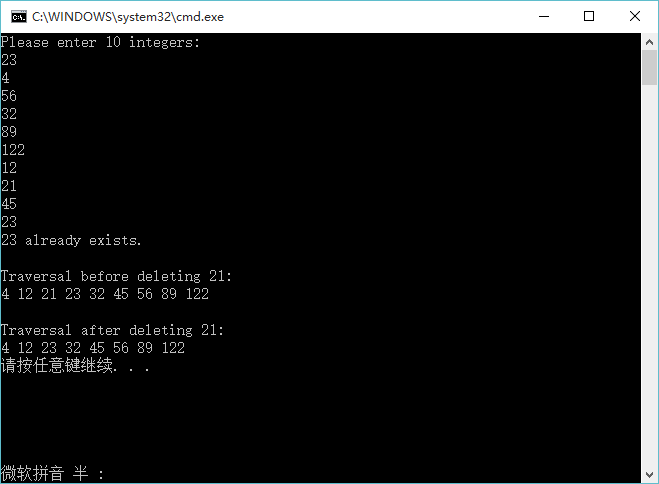
\includegraphics[width=15cm]{images/rbtreetest.png}
                \caption{红黑树插入删除测试}
                \label{fig:rbtreetest}
            \end{figure}

    \section{Windows进程地址空间的内存管理}
        \subsection{虚拟地址描述符与VAD树}
            Windows进程地址空间的范围是\texttt{0x0-0x7fffffff},进程必须经过“保留(Reserve)”和“提交(Commit)”两个阶段,才能使用一段地址范围。因此对于进程地址空间中的任何一个页面地址范围,它一定处于三种状态之一:空闲、保留、已提交。为了管理虚拟地址空间的状态,Windows中提出了VAD(虚拟地址描述符,Virtual Address Descriptor)。对于每一个进程,Windows的内存管理器维护一组VAD来描述一段被分配进程虚拟地址空间的状态\cite{ModernOS}。
            
            为了提高查找效率,Windows中的VAD被组织成一棵AVL树,进程EPROCESS对象中的VadRoot域指向此树的根,以下是VadRoot的类型MM\_AVL\_TABLE以及VAD树中结点类型MMADDRESS\_NODE的定义\cite{WinKernel}:
\begin{lstlisting}[language={C}]
typedef struct _MMADDRESS_NODE {
    union {
        LONG_PTR Balance : 2;
        struct _MMADDRESS_NODE *Parent;
    } u1;
    struct _MMADDRESS_NODE *LeftChild;
    struct _MMADDRESS_NODE *RightChild;
    ULONG_PTR StartingVpn;
    ULONG_PTR EndingVpn;
} MMADDRESS_NODE, *PMMADDRESS_NODE;
typedef struct _MM_AVL_TABLE {
    MMADDRESS_NODE BalancedRoot;
    ULONG_PTR DepthOfTree: 5;
    ULONG_PTR Unused: 3;
#if defined (_WIN64)
    ULONG_PTR NumberGenericTableElements: 56;
#else
    ULONG_PTR NumberGenericTableElements: 24;
#endif
    PVOID NodeHint;
    PVOID NodeFreeHint;
} MM_AVL_TABLE, *PMM_AVL_TABLE;
\end{lstlisting}

            在MMADDRESS\_NODE结构中,Balance、Parent、LeftChild和RightChild用于维护AVL树本身,StartingVpn和EndingVpn则记录了一个结点对应的虚拟地址范围。
            
            需要注意的是,MM\_AVL\_TABLE中的BalancedRoot是一个内嵌的MMADDRESS \\ \_NODE类型结构体,真正的根节点应该位于它的右子树RightChild。
            
        \subsection{Windows中的AVL树实现}
            WRK中的AVL树实现代码位于$\mathtt{\backslash WRK \backslash base \backslash ntos \backslash mm \backslash addrsup.c}$,其中实现了插入结点(MiInsertNode)、删除结点(MiRemoveNode)、寻找结点或其父结点(MiFindNodeOrParent)、检查冲突结点(MiCheckForConflictingNode)和AVL树平衡调整(MiRebalanceNode)等函数。前三个函数通常会被其他模块调用,其原型如下:
\begin{lstlisting}[language={C}]
VOID FASTCALL MiInsertNode (
    IN PMMADDRESS_NODE NodeToInsert,
    IN PMM_AVL_TABLE Table
);
VOID FASTCALL MiRemoveNode (
    IN PMMADDRESS_NODE NodeToDelete,
    IN PMM_AVL_TABLE Table
);
TABLE_SEARCH_RESULT MiFindNodeOrParent (
    IN PMM_AVL_TABLE Table,
    IN ULONG_PTR StartingVpn,
    OUT PMMADDRESS_NODE *NodeOrParent
);
\end{lstlisting}
        
        插入新结点时,需要调用MiFindNodeOrParent确认新结点的插入位置。插入或删除结点后,需要通过MiRebalanceNode调整AVL树的平衡。
            
        \subsection{Windows中的红黑树实现}
            Windows中的AVL树每个结点都有Balance域,记录当前结点的平衡因子。将AVL树替换为红黑树时,可以继续使用Balance域,用于记录结点的颜色。考虑到Windows中的AVL树结点初始化时的平衡因子为0,而红黑树需要将结点的颜色初始化为黑色,因此将黑色定义为0,红色定义为1。
            
            AVL树和红黑树的查找操作基本一致,因此需要修改的代码大都和树的组织有关。\texttt{Linux Kernel}中的红黑树实现非常优秀,对结点类型和相关操作稍作修改,即可适应WRK中的VAD树\footnote{修改后的代码见附件$\mathtt{\backslash codes\backslash addrsup.c}$。}。
            
            \subsubsection{宏定义}
                红黑树中颜色的定义和查询颜色、设置颜色、查询父结点的操作比较简单,可以直接通过宏定义完成。
\begin{lstlisting}[language={C}]
#define RB_RED 1
#define RB_BLACK 0
#define rb_parent(r) (SANITIZE_PARENT_NODE(r->u1.Parent))
#define rb_color(r) ((r)->u1.Balance)
#define rb_is_red(r) (rb_color(r))
#define rb_is_black(r) (!rb_color(r))
#define rb_set_black(r) do {(r)->u1.Balance = RB_BLACK;} while(0)
#define rb_set_red(r) do {(r)->u1.Balance = RB_RED;} while(0)      
\end{lstlisting}      
            
            \subsubsection{树的调整操作}
                树的调整操作包括设置父结点(rb\_set\_parent)、连接两个结点(rb\_link\_node)、左旋 \\
                (\_\_rb\_rotate\_left)、右旋(\_\_rb\_rotate\_right)、插入颜色(rb\_insert\_color)、擦除颜色 \\
                (\_\_rb\_erase\_color)。这些函数可以直接从\texttt{Linux Kernel}中移植。需要将节点类型修改为MMADDRESS\_NODE,并修改相应的父结点地址、结点颜色的操作部分。
            
            \subsubsection{结点插入}
                在MiInsertNode函数中先调用MiFindNodeOrParent函数确定新节点的插入位置,根据MiFindNodeOrParent返回值不同进行如下操作:
                \begin{description}
                  \item[返回TableEmptyTree] 将新结点作为VAD树的根,无需调整平衡,即:
\begin{lstlisting}[language={C}]
Table->BalancedRoot.RightChild = NodeToInsert;
rb_set_parent(NodeToInsert,&Table->BalancedRoot);
\end{lstlisting}
                  \item[返回TableInsertAsLeft] 将新结点插入到NodeOrParent的左子树;
                  \item[返回TableInsertAsRight] 将新结点插入到NodeOrParent的右子树,后两种情况需要调用rb\_insert\_color调整平衡:
\begin{lstlisting}[language={C}]
if (SearchResult == TableInsertAsLeft)
{
	NodeOrParent->LeftChild = NodeToInsert;
}
else
{
	NodeOrParent->RightChild = NodeToInsert;
}
rb_link_node(NodeToInsert, NodeOrParent);
rb_insert_color(NodeToInsert, Table);
\end{lstlisting}
                \end{description}
                
                插入新结点后,还需要将Table->NumberGenericTableElements计数器的值加1。
            
            \subsubsection{结点删除}
                \texttt{Linux Kernel}中提供了结点删除函数rb\_erase,因此只需要在MiRemoveNode函数中调用rb\_erase,并将Table->NumberGenericTableElements的值减1。
                
                由于红黑树已经实现了自己的旋转和颜色调整方法,WRK中的MiRebalanceNode、MiPromoteNode函数不再需要,可以删除。

    \section{实验结果}
        将编译后的内核程序\texttt{wrkx86.exe}放入虚拟机,重新启动后选择\texttt{Windows Server 2003, WRK}启动项,可以正常启动系统。

        在宿主机中打开\texttt{WinDbg},进入内核调试,然后使用调试模式启动虚拟机,再启动一个程序(如记事本)。在\texttt{WinDbg}中使用\texttt{!process 0 0}命令查看所有进程,记录下\texttt{notepad.exe}的CID,然后使用\texttt{!process CID 1}命令查看\texttt{notepad.exe}的VAD树根结点地址,再使用\texttt{!vad addr}即可查看\texttt{notepad.exe}的VAD树\cite{WinInternal},结果如图\ref{fig:vad4notepad}所示。
        \begin{figure}[htb]
            \centering
            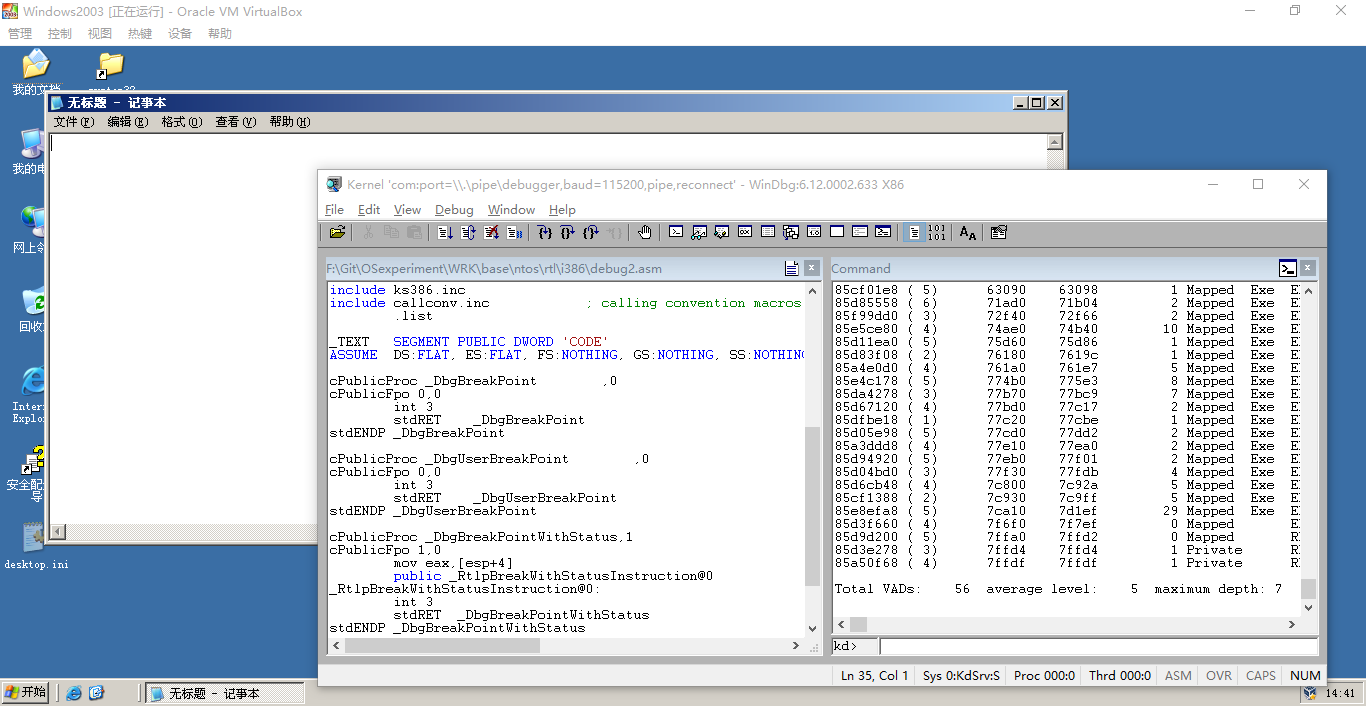
\includegraphics[width=\textwidth]{images/vad4notepad.png}
            \caption{替换内核后运行系统并查看进程的VAD树}
            \label{fig:vad4notepad}
        \end{figure}

        使用红黑树实现的VAD树在Windows Server 2003中运行正常。

    \section{实验总结}
        实验指导书中提到本实验“涉及操作系统源代码的修改,难度较大”。本次实验前后共计用时4天,由于        \texttt{Linux Kernel}中提供了代码风格良好的红黑树实现,我真正用于写代码的时间大约只有半天,而花费在\texttt{Windows 2003 SP1}的安装配置、WRK源代码结构和VAD树相关函数的理解、\texttt{Source Insight}和\texttt{WinDbg}的使用等方面的时间占据了绝大多数,我想这才是实验的真正难点所在。
        
        \texttt{Linux Kernel}的代码风格、注释和文档让我感到惊异,开源社区的协作使得一个复杂软件的每一个细节都如此精致,详细的注释和文档让我很快就理解了红黑树的实现原理,并通过简单修改得到了独立的红黑树程序。阅读WRK代码的过程则明显不如\texttt{Linux Kernel}顺利,我在图书馆借阅了两本\texttt{Windows}内核相关书籍,借助\texttt{Source Insight}强大的符号引用管理功能,才理清了WRK的结构,并在\texttt{addrsup.c}文件中分离出需要修改的函数。
        
        这次实验让我对操作系统的内存管理有了更深入的认识,阅读和理解操作系统内核源代码的过程也让我对操作系统产生了浓厚的兴趣,希望自己能有机会在开源社区中贡献一份力量。

    \bibliographystyle{plain}
    \bibliography{ref.bib}
\end{document} 